\documentclass{article}
\usepackage{amsmath}
\usepackage{amssymb}
\usepackage{dsfont}
\usepackage{unicode-math}
\numberwithin{equation}{section}
\numberwithin{figure}{section}
\usepackage{graphicx}
\graphicspath{{./images/}}

\usepackage{pdfpages}
\usepackage{verbatim}
\usepackage{xeCJK}
\usepackage{hyperref}
%\usepackage{apacite}
\usepackage{natbib}
\usepackage{grffile}
\usepackage{listings}
\lstset{
 columns=fixed,       
 numbers=left,                                        % 在左侧显示行号
 numberstyle=\tiny\color{gray},                       % 设定行号格式
 frame=single,                                          % 不显示背景边框
 keywordstyle=\color[RGB]{40,40,255},                 % 设定关键字颜色
 numberstyle=\footnotesize\color{darkgray},           
 commentstyle=\it\color[RGB]{0,96,96},                % 设置代码注释的格式
 stringstyle=\rmfamily\slshape\color[RGB]{128,0,0},   % 设置字符串格式
 showstringspaces=true,                              % 显示字符串中的空格
 language=c++,                                        % 设置语言
}
\hypersetup{
    colorlinks=true,
    linkcolor=blue,
    filecolor=magenta,
    urlcolor=cyan,
}
%--------Commands for local pdf reference------%
\newcommand{\citeint}[2]{\cite{#1}\hyperlink{./references/#1.pdf.#2}{(P#2)}}
\newcommand{\citeext}[2]{\href[page=#2]{../references/#1.pdf}{(P#2)}}
\newcommand{\citeinclude}[1]{\includepdf[link=true,pages=-,fitpaper=true]{./references/#1.pdf}}
%--------Commands/Operators for math------%
\DeclareMathOperator*{\argmax}{argmax}
\DeclareMathOperator*{\argmin}{argmin}
%--------Environments for math------------%
\newcounter{topic}[subsection]
\newenvironment{defi}{\refstepcounter{topic}\label{\thesubsection.\thetopic}\par\medskip
   \noindent \textbf{Definition~\thesubsection.\thetopic~} \rmfamily }{ \medskip}
\newenvironment{theo}{\refstepcounter{topic}\label{\thesubsection.\thetopic}\par\medskip
   \noindent \textbf{Theorem~\thesubsection.\thetopic~} \rmfamily }{\medskip}
\newenvironment{coro}{\refstepcounter{topic}\label{\thesubsection.\thetopic}\par\medskip
   \noindent \textbf{Corollary~\thesubsection.\thetopic~} \rmfamily }{ \medskip}
\newenvironment{lemm}{\refstepcounter{topic}\label{\thesubsection.\thetopic}\par\medskip
   \noindent \textbf{Lemma~\thesubsection.\thetopic~} \rmfamily }{ \medskip}
\newenvironment{exam}[1]{\refstepcounter{topic}\label{\thesubsection.\thetopic}\par\medskip
   \noindent \textbf{Example~\thesubsection.\thetopic~} \rmfamily }{ \medskip}

\newenvironment{rema}[1]{\refstepcounter{topic}\label{\thesubsection.\thetopic}\par\medskip
   \noindent \textbf{Remark~\thesubsection.\thetopic~} \rmfamily }{ \medskip}
\newenvironment{prof}{\par\medskip \noindent \textit{Proof.}~\rmfamily}{\medskip}
\title{Overview of Reinforcement Learning}
\author{陈辉}
\date{}
\begin{document}
\maketitle
\tableofcontents
\newpage


\part{Reinforcement Learning An Introduction}
\setcounter{section}{0}
\section{Introduction}
\subsection{Reinforcement Learning}
\section{Multi-armed Bandits}
This chapter mainly concerns about \textit{nonassociative evaluative feedback problems}
\subsection{A k-armed Bandit Problem}
\citeext{Reinforcement_Learning_An_Introduction}{48}
\begin{equation*}
        q_*(a) \doteq \mathds{E}[R_t | A_t = a]
\end{equation*}
Then we \textit{explore}(with $\epsilon$-greedy) to estimate this expectation and \textit{exploit} the current optimal actions.

\subsection{Action-value Methods}
Averaging the rewards:$Q_t(a)$.\\
\subsection{The 10-armed Testbed}
\citeext{Reinforcement_Learning_An_Introduction}{50}

\subsection{Incremental Implementation}
\begin{equation*}
        Q_{n+1} = Q_n + \frac{1}{n} [ R_n - Q_n]
\end{equation*}
It's called \textit{sample-avarage}.\\
A simple bandit algorithm\citeext{Reinforcement_Learning_An_Introduction}{54}

\subsection{Tracking a Nonstationary Problem}
\textit{Nonstatinary} means the reward probabilities change over time. Thus we should concentrate more on recent rewards than long-past rewards.
\begin{align*}
        Q_{n+1} &= Q_n + \alpha[R_n - Q_n]\\
                &= (1-\alpha)^n Q_1 + \sum_{i=1}^{n}\alpha(1-\alpha)^{n-i} R_i.
\end{align*}
It's called an \textit{exponential recency-weighted average}.\\
Convergence conditions:
\begin{equation*}
        \sum_{n=1}^{\infty} \alpha_n(a) = \infty, \text{and} 
        \sum_{n=1}^{\infty} \alpha_n^2(a) < \infty
\end{equation*}
Respectively, $\alpha_n(a) = \frac{1}{n}$ converges, while constant $\alpha$ does not. Instead its Q value varys according to recent rewards.\\

\subsection{Optimistic Initial Values}
\subsection{Upper-Confidence-Boundd Action Selection}
\begin{equation*}
        A_t \doteq \argmax_a [Q_t(a)+c \sqrt{\frac{\log t}{N_t(a)}}]
\end{equation*}
\subsection{Gradient Bandit Algorithms}
\textit{soft-max distribution}
\begin{equation*}
        P\{A_t = a\} \doteq \frac{e^{H_t{a}}}{\sum_{b=1}^{k} e^{H_t{b}}} = \pi _t(a)
\end{equation*}
A natural learning algorithm: 
\begin{equation*}
        H_{t+1}(a) = H_t(a) + \alpha (R_t - \bar{R_t})(\mathds{1}_{a=A_t} - \pi_t(a))
\end{equation*}
\textbf{The Bandit Gradient Algorithm as Stochastic Gradient Ascent}\citeext{Reinforcement_Learning_An_Introduction}{60}

\subsection{Associative Search}

\section{Finite Markov Decision Processes}
\subsection{The Agent-Environment Interface}
\begin{figure}
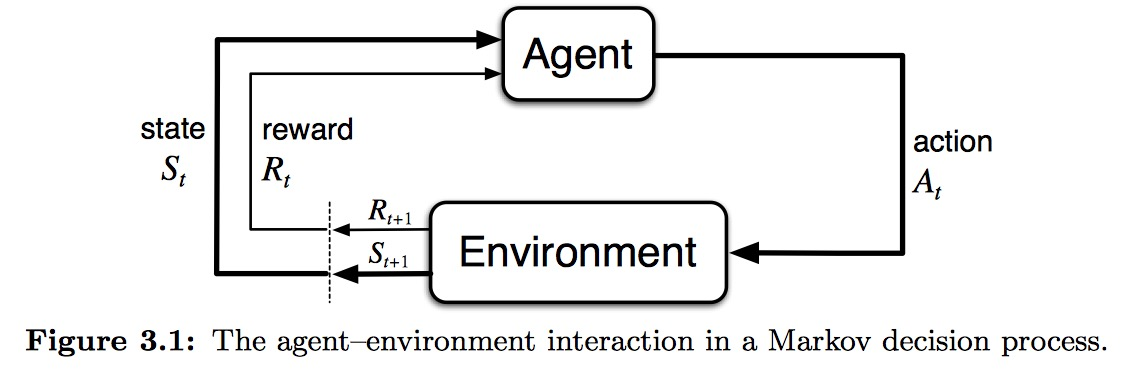
\includegraphics[width = \textwidth]{fig_3.1}
\caption{The agent-environment interaction in a MDP.}
\end{figure}

\begin{equation*}
p(s',r|s,a) \doteq Pr\{S_t=s',R_t=r | S_{t-1}=s,A_{t-1}=a\}
\end{equation*}
\textit{Markov property}\\
In MDP, the probability of each possible value for $S_t$ and $R_t$ depends only on the immmediately preceding state and action. The current state include the whole past information.








\part{Best Articles}
\section{Playing Atari with Deep Reinforcement Learning}
\subsection{Introduction}
\subsection{Background}
Basic denotes:
\begin{align*}
    \mathcal{E} &: \text{The environment.}\\
    a_t &: \text{Actions at time t.}\\ 
    x_t &: \text{Observations which are raw pixels.}\\
    r_t &: \text{Rewards at time t.}\\
\end{align*}
Note that any rewards may depend on the whole prior sequence(or a long enough prior sequence). Thus we define:
\begin{align*}
        s_t &: = {x_1,a_1,\dots,a_{t-1},x_t}.\\
\end{align*}
And the future discounted return:
\begin{equation*}
        R_t = \sum_{t'=t}^T \gamma^{t'-t} r_{t'}
\end{equation*}
where T denotes the time-step at which the game terminates.\\
Thus we have the optimal action-value function:
\begin{equation*}
        Q^*(s,a)= \max_{\pi} \mathds{E}_{s'\sim\mathcal{E}}R_t
\end{equation*}
\subsubsection*{Bellman Equation}
Basic intuition:` if the optimal value $Q^*(s',a')$ of the sequence s' \textcolor{red}{at the next time-step was known for all possible actions a'}, then
\begin{equation}
        Q^*(s,a) = \mathds{E}_{s' \sim \mathcal{E}}[ r + \gamma max_{a'}Q^*(s',a')|s,a ]
\end{equation}
We use a function to 





\bibliographystyle{plain}
\bibliography{overview_RL}

\citeinclude{Playing_Atari_with_Deep_Reinforcement_Learning}
\citeinclude{Asynchronous_Methods_for_Deep_Reinforcement_Learning}
\end{document}


%\includepdf[link=true,pages=-,fitpaper,angle=-90]{./papers/<++>.pdf}
